\section{Working principles of disk brake systems}\label{sec:working-principles-of-disk-brake-systems}

		In general terms, a disc break can be summarized as a type of brake that uses calipers to squeeze pairs of pads against a disc coupled to a shaft in order to create friction. This generated friction ought to retard the rotation of this shaft coupled to the disk. A moving car, or being more specific, a rotating shaft has a certain amount of kinetic energy, the brakes of a car are designed to convert this kinetic energy to heat (through friction) in order to decelerate the car \cite{limpert1999brake}. Figure \ref{fig:working-of-disk-breaks} shows a schematic for a typical disk break.

		\begin{figure}[htbp]
			\centering
				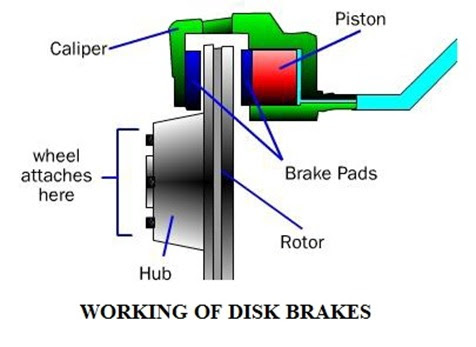
\includegraphics[scale=0.55]{figuras/fig-disk_brake_working}
			\caption{Schematic for disk brake systems \cite{fig-working-of-disk-breaks}}
			\label{fig:working-of-disk-breaks}
		\end{figure}

		As Figure \ref{fig:working-of-disk-breaks} shows, some of the main components of a typical disk brake system and their respective functions are \cite{carparts-brake}:

		\begin{itemize}
			\item\textit{Caliper}: Fits over the rotor like a clamp, houses the pads and pistons. This part does not tend to wear out quickly, usually, damages on this part are caused by using outworn pads or disks \cite{goodyear-calipers}.\label{itm:caliper}
			\item\textit{Pads}: There are two brake pads on each caliper, this is the part that is effectively in contact with the disk. Pads are used in order to prevent disk wear and caliper wear, this parts are made with specific materials that provide better perfomance, hence more friction with less dissipated heat. Pads tend to wear out quickly in a vehicle and should be checked and replaced quite often.\label{itm:pads}
			\item\textit{Piston}: Most of brake discs are activated through a hydraulic mechanism, when the break pedal is pressed the brake fluid goes to the piston and the piston squeezes the to brake pads against the disk.\label{itm:piston}
			\item\textit{Rotor}: The disk rotor is the main component of the system, it is directly connected to the wheel's shaft. The rotor wears with time, if break pads are replaced accordingly the rotor tends to last more than the pads. Usually a vehicle will undergo more than one brake pads replacement before having its disks replaced. \label{itm:rotor}
		\end{itemize}